% Don't touch this %%%%%%%%%%%%%%%%%%%%%%%%%%%%%%%%%%%%%%%%%%%
\documentclass[addpoints]{exam}
\usepackage{fullpage}
\usepackage[left=1.0in,top=1.0in,right=1.0in,bottom=1.0in,headheight=3ex,headsep=3ex]{geometry}
\usepackage{graphicx}
\usepackage{float}
\usepackage{adjustbox}
\usepackage{comment}
\usepackage{tikz}
\usetikzlibrary{calc}
\usetikzlibrary{matrix}
\usetikzlibrary{positioning}
\usepackage{amsmath}

\tikzset{   
	every picture/.style={remember picture,baseline},
	every node/.style={anchor=base,align=center,outer sep=1.5pt},
	every path/.style={thick},
}
\newcommand\marktopleft[1]{%
	\tikz[overlay,remember picture] 
	\node (marker-#1-a) at (-.3em,.3em) {};%
}
\newcommand\markbottomright[2]{%
	\tikz[overlay,remember picture] 
	\node (marker-#1-b) at (0em,0em) {};%
}
\tikzstyle{every picture}+=[remember picture] 
\tikzstyle{mybox} =[draw=black, very thick, rectangle, inner sep=10pt, inner ysep=20pt]
\tikzstyle{fancytitle} =[draw=black,fill=red, text=white]


\usepackage{graphicx,stackengine,xcolor}
\newcommand\Circle[1]{%
	\def\useanchorwidth{T}%
	\def\stacktype{L}%
	\stackon[0pt]{#1}{\scalebox{2.0}[1.15]{\textcolor{red}{$\bigcirc$}}}%
}
\newcommand{\blankline}{\quad\pagebreak[2]}
%%%%%%%%%%%%%%%%%%%%%%%%%%%%%%%%%%%%%%%%%%%%%%%%%%%%%%%%%%%%%%

% Modify Course title, instructor name, semester here %%%%%%%%

\title{ECN 453: Final Exam}
% Modify header here %%%%%%%%%%%%%%%%%%%%%%%%%%%%%%%%%%%%%%%%%
\rhead{\footnotesize ECN 453: Final Exam}

\date{} 

\begin{document}
	\maketitle
	\begin{center}
		\fbox{\fbox{\parbox{6in}{\centering\
					\textbf{Instructions}:
					\begin{itemize}
					\item You have \textbf{110 minutes}
					\item Please write your final answer in the underlined section (where provided). 
					\item You may bring a calculator and notes on two, two-sided cheat-sheets, on letter-size paper. 
					\item Please be neat. If your work is too messy it will not be graded.
					\item Be sure to show your working.
					\item This is a long exam, so there are lots of ways to get points. If you get stuck, move on!
					\item Good luck!
					\end{itemize}	
			}}}
	\end{center}
	
	\vspace{5mm}
	\makebox[0.75\textwidth]{Name: \enspace\hrulefill}
	\vspace{50pt}
	\begin{center}
		\gradetable[h][questions]
	\end{center}
	
	\newpage
	
\begin{questions}
	\subsection*{Short Answer Questions (45 points)}
	\vspace{11pt}
	\question Depending on the question, write either: 
	\begin{itemize}
		\item a number 
		\item one of: True, False, or NEI (Not Enough Information)
		\item a definition or an example (i.e. one or a few words)
	\end{itemize}
	\vspace{11pt}
	\begin{parts}
		\part[3] If entry costs are endogenous, then the equilibrium number of firms is less sensitive to changes in market size than if entry costs are exogenous.
		
		\answerline[answer]
		
		\part[3]  Give one reason why, in reality, observed market structure might depart from the simple theoretical example we discussed in class.
		\answerline[answer]
		
		\part[3] Suppose there is an upstream manufacturer $M$ selling an input to two downstream retailers $R_1$ and $R_2$ (and these downstream retailers are competing against each other). If the manufacturer merges with $R_1$, would you expect the downstream price of $R_1$ ($p_1$) to \textit{increase, decrease, or is the effect ambiguous,} compared to vertical separation?
		
		\answerline[answer]
		
		\part[3] Consider again the merger in the previous question. Give the reason discussed in class why we would expect the downstream price between $M$ and $R_2$ to increase, compared to vertical separation?
		
		\answerline[answer]
		
		\part[3] True, False, or Not Enough Information: Suppose that two firms choose to become one firm using a horizontal merger. This merger will \textit{always} increase the joint profits of the merging firms.
		
		\answerline[answer]
		
		\part[3] Put yourself in the position of a lawyer trying to convince a judge to approve the 1996 Staples and Office Depot merger discussed in class. Would you argue that Staples and Office Depot compete using a (i) broad market definition (e.g. stores that sell office supplies) or (ii) a narrow market definition (e.g. office superstores)?
		
		\answerline[answer]
		
		\part[3] Suppose there are three firms in a market with market shares 0.4, 0.3, and, 0.3, respectively. Compute the Herfindahl-Hirschman Index.

		\answerline[answer]
		
		\part[3] What is the value of the Lerner index under perfect competition?
		
		\answerline[answer]
		
		\part[3] What is the value of the Herfindahl–Hirschman Index under monopoly?

		\answerline[answer]
				
		\part[3] Consider an identical n-firm Cournot market with market size $S=1$, total demand $p=20-Q$ (where Q is the total market quantity), and the total cost for each firm is $C(q)=2+2q$. Assuming that firms continue to enter so long as profit is not negative, how many firms will enter the market in equilibrium?
		\answerline[answer]

		\part[3] Consider an identical n-firm Cournot market with market size $S=1$, total demand $p=15-Q$ (where Q is the total market quantity), and the total cost for each firm is $C(q)=2+q$. Assuming that firms continue to enter so long as profit is not negative, what is the equilibrium price?
	\answerline[answer]
		
		\part[3] True, False, or Not Enough Information: Consider an identical n-firm Cournot market with market size $S=1$ and exogenous entry costs. Suppose that the market size doubles so that $S=2$. Then, the equilibrium number of firms in the market will double.
		\answerline[answer]
		
		\part[3] Give an example of a \textit{unilateral effect} of a merger.
		\answerline[answer]

		\part[3] Give an example of an endogenous entry cost.
		\answerline[answer]

		\part[3] True, False, or Not Enough Information: Provide one benefit (that we discussed in class) that a regulator might consider when deciding whether to approve a merger.
		\answerline[answer]

	\end{parts}
	
	\newpage
	\subsection*{Movie Theater Question (30 points)}
	\question Suppose you are the owner of a movie theater. There are two types of customers: students (denoted `s') and non-students (denoted `ns'). The demand for movie seats for each of these segments is:
	\begin{align*}
		\text{Student: } &q_{s} = 80 - 2p_{s} \\
		\text{Non-student: }& q_{ns} = 85 - p_{ns}
	\end{align*}
	\begin{parts}
		\part [30] Assume that you cannot distinguish between students and non-students, and so you can only set a single \textit{uniform price} for all consumers. Assume that the marginal cost of a seat is \$15. What is the optimal uniform price? 
		\vspace{500pt}
		\answerline[answer] 
	\end{parts}
	
	\subsection*{Stackelberg Competition (30 points)}
	\question There are two firms in a market with total demand $p=100-Q$. Firm 1 in an incumbent and so moves first. Firm 2 is a potential entrant and so moves second. Firm 1's total cost is $C(q_1)=q_1^2$.  Firm 2's total cost is $C(q_2)=4q_2$. 
	\vspace{11pt}
\begin{parts}
	\part[15] Suppose that the firms compete in a Stackelberg equilibrium. What is the equilibrium quantity for \underline{Firm 1}?
	\vspace{500pt}
	\answerline[answer]
	\newpage
	\part[15] Suppose now that Firm 2 (the potential entrant) now chooses whether to enter after Firm 1 makes its production decision. If Firm 2 enters then it pays an entry cost $E=16$. Which values of $q_1$ deter Firm 2's entry?
	\vspace{500pt}
	\answerline[answer]
\end{parts}

\newpage
	\subsection*{Hotelling Model (30 points)}
\question Suppose 100 consumers are uniformly distributed on a 1 mile stretch of road. There are two supermarkets on the road: Supermarket 1 is located at the west end of the road (at location = 0), and Supermarket 2 is part way along the road (at location = 0.6). Transport costs for consumers are \underline{\$1.0 per mile}. The supermarkets' marginal costs are 0. The supermarkets compete on prices: denote Supermarket 1's price $p_1$ and Supermarket 2's price $p_2$.
\begin{parts}
	\part[15] What is the demand for each supermarket?\footnote{When computing consumer choices, only consider the transport costs to get to the supermarket, don't worry about the return journey.}
	\vspace{500pt}
	\answerline[answer]
	\newpage
	\part[15] What are the equilibrium prices?
	\vspace{600pt}
	\answerline[answer]
	%\part[10] Suppose that prices are fixed. A third supermarket (Firm 3) enters the market and can choose where on the road to locate. Explain in one to two sentences: where on the road will this new supermarket choose to locate?
	%\vspace{250pt}
	%\answerline[answer]
\end{parts}
	\newpage

	\subsection*{Collusion (30 points)}
\question Consider the following game and suppose that it is repeated an infinite number of times. Players have a discount value of $\delta$. Suppose that $x$ is a number.
\begin{figure}[h]
	\centering
	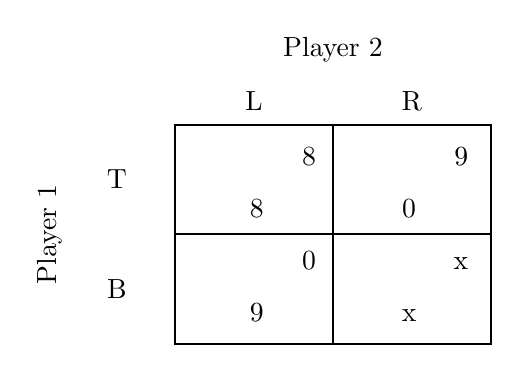
\begin{tikzpicture}
		\matrix[matrix of math nodes,
		every odd row/.style={align=right},every evenrow/.style={align=left},every node/.style={text width=1.5cm},row sep=0.2cm,column sep=0.2cm,ampersand replacement=\&] (m) {
			8\&9 \\
			8\&0 \\
			0 \&x \\
			9 \&x\\
		};
		\draw (m.north east) rectangle (m.south west);
		\draw (m.north) -- (m.south);
		\draw (m.east) -- (m.west);
		
		% Player 1
		\coordinate (c) at ($(m.north west)!0.25!(m.south west)$);
		\coordinate (d) at ($(m.north west)!0.75!(m.south west)$);
		\node[left=2pt of c,text width=1cm]  {T};
		\node[left=2pt of d,text width=1cm]  {B};
		
		% Player 2
		\coordinate (a) at ($(m.north west)!0.25!(m.north east)$);
		\coordinate (b) at ($(m.north west)!0.75!(m.north east)$);
		\node[above=5pt of a,anchor=base] {L};
		\node[above=5pt of b,anchor=base] {R};
		
		\node[above=18pt of m.north] (firm b) {Player 2};
		\node[left=1.6cm of m.west,rotate=90,align=center,anchor=center] {Player 1};
		
		%\node[above=5pt of firm b]  {Payoff Matrix};
	\end{tikzpicture}
\end{figure}

\begin{parts}
	\part[15] Suppose that \underline{x=0}. For what values of $\delta$ can collusion on (T,L) be sustained under the following grim trigger strategy:
	\begin{itemize}
		\item Play (T,L) if (T,L) has been played in all previous periods
		\item Otherwise play (B,R).
	\end{itemize}
	\vspace{300pt}
	\answerline[answer]
	\newpage
	\part[15] Suppose that $\delta=0.5$. For what values of $x$ can collusion on (T,L) by sustained using the grim  trigger strategy from Part (a)?
		\vspace{600pt}
	\answerline[answer]
\end{parts}

	\subsection*{Vertical Relationships (30 points)}
\question Suppose that there are two firms in a supply chain: a manufacturer who sells to a retailer. The timing is as follows:

\begin{enumerate}
	\item Manufacturer has a constant marginal cost $c=1$ and sets input price $w$ to maximize profit.
	\item Retailer buys input from manufacturer for price $w$. Retailer sets price $p$ to maximize profit with demand $D(p)=20-0.5p$.
\end{enumerate}
\begin{parts}
	\part[20] What are the joint profits of the firms (i.e. the sum of the profit of the manufacturer and the retailer) under vertical separation?
	\vspace{500pt}
	\answerline[answer]
	\part[10] What two-part tariff (paid by the retailer to the manufacturer) will induce the vertically separated firms to jointly achieve the profits from vertical integration?

	\vspace{600pt}
		\answerline[answer]
	%\answerline[answer]
\end{parts}
\end{questions}

\end{document}